\documentclass[border=3pt,tikz]{standalone}
\usepackage{bm,amsmath}
\usetikzlibrary{patterns,decorations.pathmorphing,decorations.text}
\usetikzlibrary{arrows.meta}
\usetikzlibrary{calc}


\begin{document}

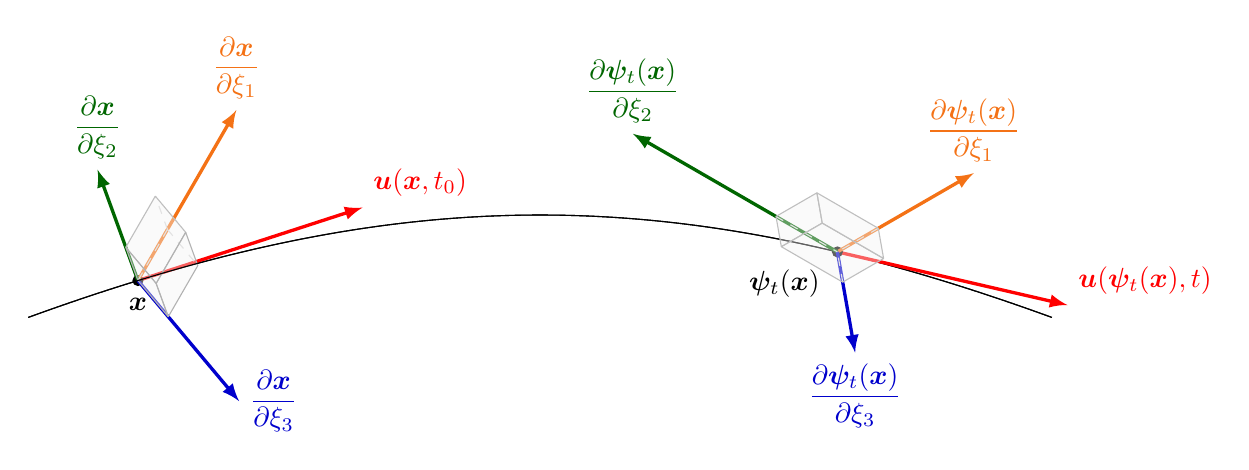
\begin{tikzpicture}[scale=1]
    \colorlet{mydarkblue}{blue!80!black}
    \colorlet{myblue}{blue!30}
    \colorlet{mylightblue}{blue!5}
    \colorlet{mydarkred}{red!90!black}
    \colorlet{myred}{red!30}
    \colorlet{mydarkgreen}{green!40!black}
    \colorlet{mygreen}{green!30}
    \colorlet{mydarkorange}{yellow!40!red}
    \colorlet{myorange}{yellow!80!red}
    \colorlet{myyellow}{yellow!80}
    \colorlet{mygrey}{black!15}
    \colorlet{mydarkgrey}{black!70}

    % origin
    \coordinate (O) at (0,0);

    % xyz triplet
    % \draw[-latex] (O)--++(0:1) node[right] {$\bm{\hat{x}}$};
    % \draw[-latex] (O)--++(90:1) node[above] {$\bm{\hat{y}}$};
    % \draw[-latex] (O)--++(225:0.8) node[below left] {$\bm{\hat{z}}$};


    % POINT t_0

    % points for drawing the flow curve
    \coordinate (X_path_start) at ($(O)+(-1,2)$);
    \coordinate (X_path_end) at ($(O)+(12,2)$);

    % define x_t and velocity at x_t
    \draw (X_path_start) to[bend left=20] coordinate[pos=0.1] (X_t) (X_path_end);
    \draw[-latex,very thick,red] (X_t)--++(18:3) node[above right,pos=1] {$\bm{u}(\bm{x},t_0)$};
    \fill (X_t) circle (2pt) node[below=0.1cm] {$\bm{x}$};
    
    % define \xi_1-curve and vector
    \draw[-latex,mydarkorange,very thick] (X_t) -- coordinate[pos=0.3] (dxi_1) ++(60:2.5) node[above,pos=1] {$\begin{aligned}\frac{\partial\bm{x}}{\partial \xi_1}\end{aligned}$};
    
    % define \xi_2-curve and vector
    \draw[-latex,mydarkgreen,very thick] (X_t) -- coordinate[pos=0.3] (dxi_2) ++(110:1.5) node[above,pos=1] {$\begin{aligned}\frac{\partial\bm{x}}{\partial \xi_2}\end{aligned}$};
    
    % define \xi_3-curve and vector
    \draw[-latex,mydarkblue,very thick] (X_t) -- coordinate[pos=0.3] (dxi_3) ++(-50:2) node[right,pos=1] {$\begin{aligned}\frac{\partial\bm{x}}{\partial \xi_3}\end{aligned}$};

    % draw box faces
    \draw[dashed,mygrey] (dxi_1)--($(dxi_1)+(dxi_2)-(X_t)$);
    \draw[dashed,mygrey] (dxi_1)--(X_t);
    \draw[dashed,mygrey] (dxi_1)--($(dxi_3)+(dxi_1)-(X_t)$);
    
    \draw[gray!50,fill=gray!10,fill opacity=0.4,line join=bevel] (dxi_2)--($(dxi_2)+(dxi_1)-(X_t)$)--($(dxi_3)+(dxi_2)-(X_t)+(dxi_1)-(X_t)$)--($(dxi_3)+(dxi_2)-(X_t)$)--cycle;
    
    \draw[gray!60,fill=gray!10,fill opacity=0.4,line join=bevel] (X_t)--(dxi_2)--($(dxi_2)+(dxi_3)-(X_t)$)--(dxi_3)--cycle;

    \draw[gray!60,fill=gray!10,fill opacity=0.4,line join=bevel] (dxi_3)--($(dxi_3)+(dxi_1)-(X_t)$)--($(dxi_3)+(dxi_1)-(X_t)+(dxi_2)-(X_t)$)--($(dxi_3)+(dxi_2)-(X_t)$)--cycle;


    % POINT t

    % points for drawing the flow curve
    \coordinate (X_path_start) at ($(O)+(-1,2)$);
    \coordinate (X_path_end) at ($(O)+(12,2)$);

    % define x_t and velocity at x_t
    \draw (X_path_start) to[bend left=20] coordinate[pos=0.8] (X_tt) (X_path_end);
    \draw[-latex,very thick,red] (X_tt)--++(-13:3) node[above right,pos=1] {$\bm{u}(\bm{\psi}_t(\bm{x}),t)$};
    \fill (X_tt) circle (2pt) node[below left=0.1cm] {$\bm{\psi}_t(\bm{x})$};
    
    % define \xi_1-curve and vector
    \draw[-latex,mydarkorange,very thick] (X_tt) -- coordinate[pos=0.3] (dxi_11) ++(30:2) node[above,pos=1] {$\begin{aligned}\frac{\partial\bm{\psi}_t(\bm{x})}{\partial \xi_1}\end{aligned}$};
    
    % define \xi_2-curve and vector
    \draw[-latex,mydarkgreen,very thick] (X_tt) -- coordinate[pos=0.3] (dxi_22) ++(150:3) node[above,pos=1] {$\begin{aligned}\frac{\partial\bm{\psi}_t(\bm{x})}{\partial \xi_2}\end{aligned}$};
    
    % define \xi_3-curve and vector
    \draw[-latex,mydarkblue,very thick] (X_tt) -- coordinate[pos=0.3] (dxi_33) ++(-80:1.3) node[below,pos=1] {$\begin{aligned}\frac{\partial\bm{\psi}_t(\bm{x})}{\partial \xi_3}\end{aligned}$};

    % draw box faces
    \draw[dashed,mygrey] (dxi_11)--(X_tt); 
    \draw[dashed,mygrey] (dxi_22)--(X_tt); 
    \draw[dashed,mygrey] (dxi_33)--(X_tt); 
    
    \draw[gray!50,fill=gray!10,fill opacity=0.4,line join=bevel] (dxi_22)--($(dxi_22)+(dxi_11)-(X_tt)$)--($(dxi_22)+(dxi_11)-(X_tt)+(dxi_33)-(X_tt)$)--($(dxi_22)+(dxi_11)-(X_tt)+(dxi_33)-(X_tt)+(X_tt)-(dxi_11)$)--cycle;
    \draw[gray!50,fill=gray!10,fill opacity=0.4,line join=bevel] (dxi_33)--($(dxi_33)+(dxi_22)-(X_tt)$)--($(dxi_33)+(dxi_22)-(X_tt)+(dxi_11)-(X_tt)$)--($(dxi_33)+(dxi_11)-(X_tt)$)--cycle;
    \draw[gray!50,fill=gray!10,fill opacity=0.4,line join=bevel] (dxi_11)--($(dxi_11)+(dxi_33)-(X_tt)$)--($(dxi_11)+(dxi_33)-(X_tt)+(dxi_22)-(X_tt)$)--($(dxi_22)+(dxi_11)-(X_tt)$)--cycle;
    

    
    
\end{tikzpicture}
\end{document}
